\begin{frame}
	\frametitle{Landscape approximation}
	\framesubtitle{\cite{Kauffman.1987}}
	
	\begin{itemize}
		\item random walk is time-consuming
		\item instead: using the first generations
		\item ''long jump'' instead a step 
		\item approximation of the landscape
	\end{itemize}
	
\end{frame}

\begin{frame}
	\frametitle{Fitness}
	
	\begin{itemize}
		\item implemented in EvoSuite
		\item ratio between:
		\begin{itemize}
			\item current fitness value
			\item maximum observed value
		\end{itemize}
		\item high ratio: good performing
		\item low ratio: bad performing
	\end{itemize}
	
\end{frame}

\begin{frame}
	\frametitle{Gradient branches}
	\framesubtitle{\cite{Shamshiri.2015}}
	
	\begin{itemize}
		\item implemented in EvoSuite
		\item Byte-code analysis
		\begin{itemize}
			\item branches with gradient
			\item branches without gradient
		\end{itemize}
		\item ratio between both
		\item high ratio: guidance
		\item low ratio: no guidance
	\end{itemize}
	
\end{frame}


\begin{frame}
	\frametitle{Neutrality Volume (NV)}
	\framesubtitle{\cite{Albunian.2020}}
	
	\begin{columns}[c]
		
		\column{.45\textwidth}
		
		\begin{itemize}
			\item neutrality of the landscape
			\item neutral: no guidance
			\item based on fitness values
			\item number of fitness changes
			\item depending on steps
			\begin{itemize}
				\item $NV_{Ratio}$
			\end{itemize}
		\end{itemize}	
	
		\column{.45\textwidth}
		\begin{figure}
			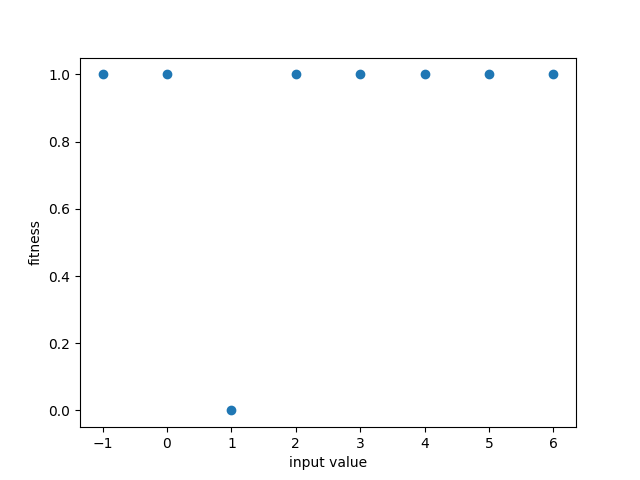
\includegraphics[width=1\textwidth]{figures/plot_no_guidance}
		\end{figure}
		
	\end{columns}	

\end{frame}

\begin{frame}
	\frametitle{Information Content (IC)}
	\framesubtitle{\cite{Vassilev.2000,Albunian.2020}}
	
	\begin{itemize}
		\item information content of the landscape
		\item ruggedness of the landscape
		\item high IC: rugged landscape
		\item low IC: soft landscape
	\end{itemize}
	
\end{frame}